\documentclass[a4paper]{article}
% Some basic packages
\usepackage{graphicx}

% Don't indent paragraphs, leave some space between them
\usepackage{parskip}

% Hide page number when page is empty
\usepackage{emptypage}
\usepackage{subcaption}
\usepackage{multicol}
\usepackage{xcolor}


% Math stuff
\usepackage{amsmath, amsfonts, mathtools, amsthm, amssymb}
% Fancy script capitals
\usepackage{mathrsfs}
\usepackage{cancel}
% Bold math
\usepackage{bm}
% Some shortcuts
\newcommand\N{\ensuremath{\mathbb{N}}}
\newcommand\R{\ensuremath{\mathbb{R}}}
\newcommand\Z{\ensuremath{\mathbb{Z}}}
\renewcommand\O{\ensuremath{\emptyset}}
\newcommand\Q{\ensuremath{\mathbb{Q}}}
\newcommand\C{\ensuremath{\mathbb{C}}}

% Easily typeset systems of equations (French package)
\usepackage{systeme}

% Put x \to \infty below \lim
\let\svlim\lim\def\lim{\svlim\limits}

%Make implies and impliedby shorter
\let\implies\Rightarrow
\let\impliedby\Leftarrow
\let\iff\Leftrightarrow
\let\epsilon\varepsilon


% horizontal rule
\newcommand\hr{
    \noindent\rule[0.5ex]{\linewidth}{0.5pt}
}

% hide parts
\newcommand\hide[1]{}

% si unitx
\usepackage{siunitx}

% Environments
\makeatother
% For box around Definition, Theorem, \ldots
\usepackage{mdframed}
\mdfsetup{skipabove=1em,skipbelow=0em}
\theoremstyle{definition}
\newmdtheoremenv[nobreak=true]{definitie}{Definitie}
\newmdtheoremenv[nobreak=true]{eigenschap}{Eigenschap}
\newmdtheoremenv[nobreak=true]{gevolg}{Gevolg}
\newmdtheoremenv[nobreak=true]{lemma}{Lemma}
\newmdtheoremenv[nobreak=true]{propositie}{Propositie}
\newmdtheoremenv[nobreak=true]{stelling}{Stelling}
\newmdtheoremenv[nobreak=true]{wet}{Wet}
\newmdtheoremenv[nobreak=true]{postulaat}{Postulaat}
\newmdtheoremenv{conclusie}{Conclusie}
\newmdtheoremenv{toemaatje}{Toemaatje}
\newmdtheoremenv{vermoeden}{Vermoeden}
\newtheorem*{herhaling}{Herhaling}
\newtheorem*{intermezzo}{Intermezzo}
\newtheorem*{notatie}{Notatie}
\newtheorem*{observatie}{Observatie}
\newtheorem*{oef}{Oefening}
\newtheorem*{opmerking}{Opmerking}
\newtheorem*{praktisch}{Praktisch}
\newtheorem*{probleem}{Probleem}
\newtheorem*{terminologie}{Terminologie}
\newtheorem*{toepassing}{Toepassing}
\newtheorem*{uovt}{UOVT}
\newtheorem*{vb}{Voorbeeld}
\newtheorem*{vraag}{Vraag}

\newmdtheoremenv[nobreak=true]{definition}{Definition}
\newtheorem*{eg}{Example}
\newtheorem*{notation}{Notation}
\newtheorem*{previouslyseen}{As previously seen}
\newtheorem*{remark}{Remark}
\newtheorem*{note}{Note}
\newtheorem*{problem}{Problem}
\newtheorem*{observe}{Observe}
\newtheorem*{property}{Property}
\newtheorem*{intuition}{Intuition}
\newmdtheoremenv[nobreak=true]{prop}{Proposition}
\newmdtheoremenv[nobreak=true]{theorem}{Theorem}
\newmdtheoremenv[nobreak=true]{corollary}{Corollary}

% End example and intermezzo environments with a small diamond (just like proof
% environments end with a small square)
\usepackage{etoolbox}
\AtEndEnvironment{vb}{\null\hfill$\diamond$}%
\AtEndEnvironment{intermezzo}{\null\hfill$\diamond$}%
% \AtEndEnvironment{opmerking}{\null\hfill$\diamond$}%

% Fix some spacing
% http://tex.stackexchange.com/questions/22119/how-can-i-change-the-spacing-before-theorems-with-amsthm
\makeatletter
\def\thm@space@setup{%
  \thm@preskip=\parskip \thm@postskip=0pt
}


% Exercise 
% Usage:
% \oefening{5}
% \suboefening{1}
% \suboefening{2}
% \suboefening{3}
% gives
% Oefening 5
%   Oefening 5.1
%   Oefening 5.2
%   Oefening 5.3
\newcommand{\oefening}[1]{%
    \def\@oefening{#1}%
    \subsection*{Oefening #1}
}

\newcommand{\suboefening}[1]{%
    \subsubsection*{Oefening \@oefening.#1}
}


% \lecture starts a new lecture (les in dutch)
%
% Usage:
% \lecture{1}{di 12 feb 2019 16:00}{Inleiding}
%
% This adds a section heading with the number / title of the lecture and a
% margin paragraph with the date.

% I use \dateparts here to hide the year (2019). This way, I can easily parse
% the date of each lecture unambiguously while still having a human-friendly
% short format printed to the pdf.

\usepackage{xifthen}
\def\testdateparts#1{\dateparts#1\relax}
\def\dateparts#1 #2 #3 #4 #5\relax{
    \marginpar{\small\textsf{\mbox{#1 #2 #3 #5}}}
}

\def\@lecture{}%
\newcommand{\lecture}[3]{
    \ifthenelse{\isempty{#3}}{%
        \def\@lecture{Lecture #1}%
    }{%
        \def\@lecture{Lecture #1: #3}%
    }%
    \subsection*{\@lecture}
    \marginpar{\small\textsf{\mbox{#2}}}
}



% These are the fancy headers
\usepackage{fancyhdr}
\pagestyle{fancy}

% LE: left even
% RO: right odd
% CE, CO: center even, center odd
% My name for when I print my lecture notes to use for an open book exam.
% \fancyhead[LE,RO]{Gilles Castel}

% \fancyhead[RO,LE]{\@lecture} % Right odd,  Left even
% \fancyhead[RE,LO]{}          % Right even, Left odd

% \fancyfoot[RO,LE]{\thepage}  % Right odd,  Left even
% \fancyfoot[RE,LO]{}          % Right even, Left odd
\fancyfoot[C]{\leftmark}     % Center

\makeatother




% Todonotes and inline notes in fancy boxes
\usepackage{todonotes}
\usepackage{tcolorbox}

% Make boxes breakable
\tcbuselibrary{breakable}

% Verbetering is correction in Dutch
% Usage: 
% \begin{verbetering}
%     Lorem ipsum dolor sit amet, consetetur sadipscing elitr, sed diam nonumy eirmod
%     tempor invidunt ut labore et dolore magna aliquyam erat, sed diam voluptua. At
%     vero eos et accusam et justo duo dolores et ea rebum. Stet clita kasd gubergren,
%     no sea takimata sanctus est Lorem ipsum dolor sit amet.
% \end{verbetering}
\newenvironment{verbetering}{\begin{tcolorbox}[
    arc=0mm,
    colback=white,
    colframe=green!60!black,
    title=Opmerking,
    fonttitle=\sffamily,
    breakable
]}{\end{tcolorbox}}

% Noot is note in Dutch. Same as 'verbetering' but color of box is different
\newenvironment{noot}[1]{\begin{tcolorbox}[
    arc=0mm,
    colback=white,
    colframe=white!60!black,
    title=#1,
    fonttitle=\sffamily,
    breakable
]}{\end{tcolorbox}}




% Figure support as explained in my blog post.
\usepackage{import}
\usepackage{xifthen}
% \pdfminorversion=7
\usepackage{pdfpages}
\usepackage{transparent}
\newcommand{\incfig}[1]{%
    \def\svgwidth{\columnwidth}
    \import{./figures/}{#1.pdf_tex}
}

% Fix some stuff
% %http://tex.stackexchange.com/questions/76273/multiple-pdfs-with-page-group-included-in-a-single-page-warning
\pdfsuppresswarningpagegroup=1


% My name
\author{S. Bettani}


\DeclareMathOperator{\length}{length}
\DeclareMathOperator{\Aut}{Aut}
\DeclareMathOperator{\diam}{diam}
\DeclareMathOperator*{\res}{res}

\title{Psicopatologia}

\begin{document}
    \maketitle
    \tableofcontents
    % start lectures
    \lecture{1}{Sun 08 Mar 2020 19:15}{Introduzione}{
Quali sono gli elementi che distinguono nell'\textbf{immaginario comune} la normalità?

\begin{enumerate}
	\item Compromissione di competenze
	\item Ricerca di aiuto
	\item Sofferenza
	\item Irrazionalità 
	\item Trasgressione 
	\item Devianza statistica
\end{enumerate}

In realtà pochi di questi criteri funziona, come il \textbf{dolore}, ma non sempre: a volte i pazienti si sentono estremamente bene (mania, ipomania, psicopatia), e a volte persone non malate soffrono.

Anche la compromissione o disabilità funziona come principio diagnostico, ed è il più utilizzato nei manuali diagnostici, ma ha dei limiti: condizioni rare possono essere vantaggiose, alcune condizioni non sono misurabili e alcune patologie possono essere normali nella società contemporanea.

\paragraph{Esempio Clinico}  

Cinzia: ragazza normale di 21 anni, ad una certa smette di uscire e di andare bene a scuola, e sta chiusa in casa tutto il giorno.

Il processo diagnostico consiste nella verifica di \textbf{ipotesi}, fermarsi troppo presto nel processo è molto rischioso
\medskip\\

\includegraphics[width=\linewidth]{./images/image1}
\medskip\\

I criteri: la presenza di più fattori è necessaria, assieme al loro covariare nel tempo.
Anche un solo episodio depressivo è sufficiente per dire che una persone ha un disturbo mentale.
Gli stessi comportamenti hanno diversi significati a diverse età.
Il contesto a volte spiega il comportamento meglio di una malattia.
Anche i fattori culturali devono essere considerati, ogni cultura ha modalità di reazione al lutto considerate normali.



    \lecture{2}{Mon 09 Mar 2020 13:41}{Definizione e Classificazione}{

\begin{itemize}
	\item Segni: indicatori di malattia osservabili
	\item Sintomi: percezione soggettiva di malessere
	\item Sindrome: covariazione di sintomi/segni, eziologia non nota
	\item Malattia: sindrome con eziologia, prognosi e decorso noti e caratteristici
\end{itemize}

In psicopatologia le l'eziologia è sempre multi fattoriale.
\medskip\\
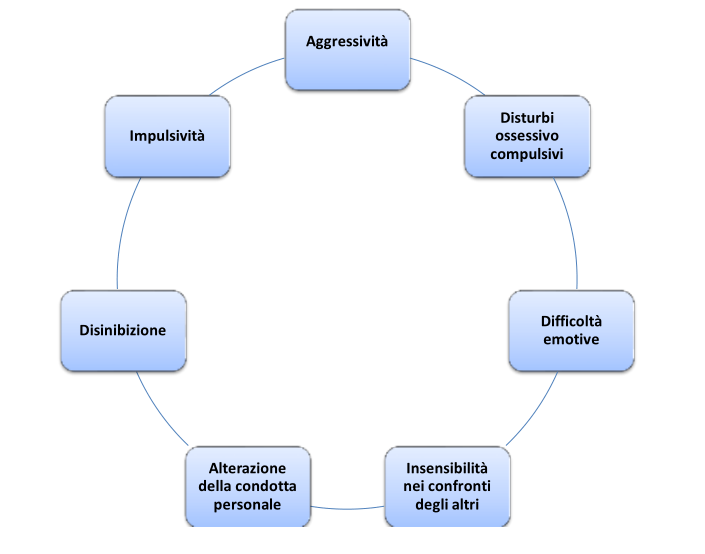
\includegraphics[width=\linewidth]{./images/image2}
\medskip\\

Secondo la visione biopsicosociale ci sono fattori:

\begin{itemize}
	\item Predisponenti
	\item Precipitanti
	\item Perpetuanti (di mantenimento) 
	\item Protettivi
\end{itemize} 
\begin{quote}
	\emph{ “La malattia mentale potrebbe (o dovrebbe) essere definita solo in presenza di dati quali: un’eziologia accertata (conoscenza delle cause e dei fattori che favoriscono o inibiscono il processo morboso); corrispondenti reperti anatomo-biologici; e rilievi patogenetici (correlazioni dimostrabili tra cause, reperti biologici ed effetti sintomatologici obiettivabili)”. }
	\begin{flushright}
		Gilberti et al., 1996
	\end{flushright}
\end{quote}

In realtà non abbiamo informazioni sulla malattia:
\medskip\\

\includegraphics[width=\linewidth]{./images/image1}
\medskip\\
Ovviamente la diagnosi non è altro che un'etichetta, un nome comune, come \emph{giraffa}, che ci dà però informazioni molto precise.

La definizione del DSM-5 del disturbo mentale è: 
\medskip\\

\includegraphics[width=\linewidth]{./images/image3}
\medskip\\
Un disturbo mentale è una sindrome caratterizzata da un’alterazione clinicamente significativa della sfera cognitiva, della regolazione delle emozioni o del comportamento di un individuo, che riflette una disfunzione nei processi psicologici, biologici o evolutivi che sottendono il funzionamento mentale.

    \documentclass[12pt, a4paper]{article}
\usepackage{graphicx}

\date{8 Gennaio 2020}
\title{None}
\author{myyuni}

\begin{document}

\maketitle

\section{}


















\end{document}

    \lecture{4}{Tue 10 Mar 2020 14:32}{La Psicopatologia Generale}{

Nel corso del tempo sono più che triplicate le diverse categorizzazioni di disturbi mentali nei DSM.

L'introduzione del DSM ha contribuito a migliorare l'\textbf{attendibilità} della diagnosi (due psichiatri diagnosticano la stessa malattia) ma la validità non è migliorata (es. Rosenhan)

Per \textbf{psicopatologia} si può intendere la psicopatologia descrittiva o interpretativa.

\paragraph{ La Psicopatologia descrittiva} si occupa dello studio e della classificazione degli elementi invarianti dei disturbi mentali, procedendo per le grandi aree dello sviluppo psicologico (percettivo, dello sviluppo, etc.), inglobando la psicopatologia \emph{oggettiva e soggettiva} 

\paragraph{La Psicopatologia oggettiva} ha come ambito d'indagine la sola realtà esterna, ed è eredità di Kraeplin, e nasce come contrapposizione all'approccio soggettivo.

\paragraph{La Psicopatologia soggettiva} ha come obiettivo la valorizzazione delle esperienze soggettive, rifiuta i metodi delle scienze naturali, fondato da Jasper. Per spiegare gli eventi interni bisogna entrare nella prospettiva empatica.

\paragraph{Il limite della comprensibilità} è raggiunto quando non sono più possibili altro che spiegazioni causali, bisogna quindi spostarsi dalla comprensione alla spiegazione.  

\paragraph{Primario/Secondario} Nel dominio della spiegazione: primario si riferisce alla causa immediata, mentre secondario si intende l'effetto. Nel dominio della comprensione primario significa inderivabile, mentre secondario ciò che emerge dal primario.

\paragraph{Variabili importanti} 
\begin{itemize}
	\item Obiettivi dell'intervento: possono essere specifici o generali
	\item Il setting 
	\item Il contratto terapeutico.
	\item Valutazione clinica
	\item Importanza attribuita alla relazione
	\item Tecniche e procedure
\end{itemize}



    \documentclass[12pt, a4paper]{article}
\usepackage{graphicx}

\date{8 Gennaio 2020}
\title{None}
\author{myyuni}

\begin{document}

\maketitle

\section{<esc>:VimtexCompile<CR>}


















\end{document}

    % end lectures
\end{document}
